% IMPORTANT: Please write various parts in different files, and then include
% them into this document.
% If you have a file called intro.tex then write: \include{intro}
% This is to avoid nasty merge conflicts, as well as to keep it tidy,
% modular, etc

\documentclass[11pt,a4paper,oneside]{report}

\usepackage{float} % have the position of pictures fixed

% Make bibliography appear in table of contents
\usepackage[nottoc,numbib]{tocbibind}

\usepackage{amsmath,amssymb,calc,ifthen,capt-of}


\usepackage[ampersand]{easylist}

\usepackage[table,usenames,dvipsnames]{xcolor} % for coloured cells in tables
\usepackage{color} % coloured text


% Allows us to click on links and references!
% http://tex.stackexchange.com/questions/73862/how-can-i-make-a-clickable-table-of-contents
\usepackage{hyperref}
\hypersetup{
    colorlinks,
    citecolor=black,
    filecolor=black,
    linkcolor=black,
    urlcolor=black
}

% Nice package for plotting graphs
% See excellent guide:
% http://www.tug.org/TUGboat/tb31-1/tb97wright-pgfplots.pdf
\usepackage{pgfplots}
\usetikzlibrary{plotmarks}
\usepackage{amsmath,graphicx}
\usepackage{epstopdf}
\usepackage{caption}
\usepackage{subcaption}

\pgfplotsset{compat = newest}

% highlight - useful for TODOs and similar
\usepackage{color}
\newcommand{\hilight}[1]{}%\colorbox{yellow}{#1}}


% margin size
\usepackage[margin=1in]{geometry}


\title{On a new metric to compare internal structures in biological networks}
\date{January 2014}
\author{
  Razvan Valentin Marinescu\\
  \texttt{rvm10@imperial.ac.uk}
}


\begin{document}
\belowdisplayskip=12pt plus 3pt minus 9pt
\belowdisplayshortskip=7pt plus 3pt minus 4pt
% General notes:

% Report Guidelines:
% http://www.doc.ic.ac.uk/lab/thirdyear/group-project/ReportGuidelines2012.pdf

% "This is more marketing than engineering. We don't want a diary"

% Tony: "How long? I don't know. Keep it short. 30 pages is absolutely fine.
% 40 a bit too much. 20 is a bit..."
% NOTE this excludes the appendices

% Keep it simple and to the point. Don't waffle

% Report is read by people who DONT know your work, though they are
% technically minded


\section*{Metabolic Networks}

\subsection*{Hsa metabolic Network (Compound-based)}


\begin{figure}[H]
  \centering
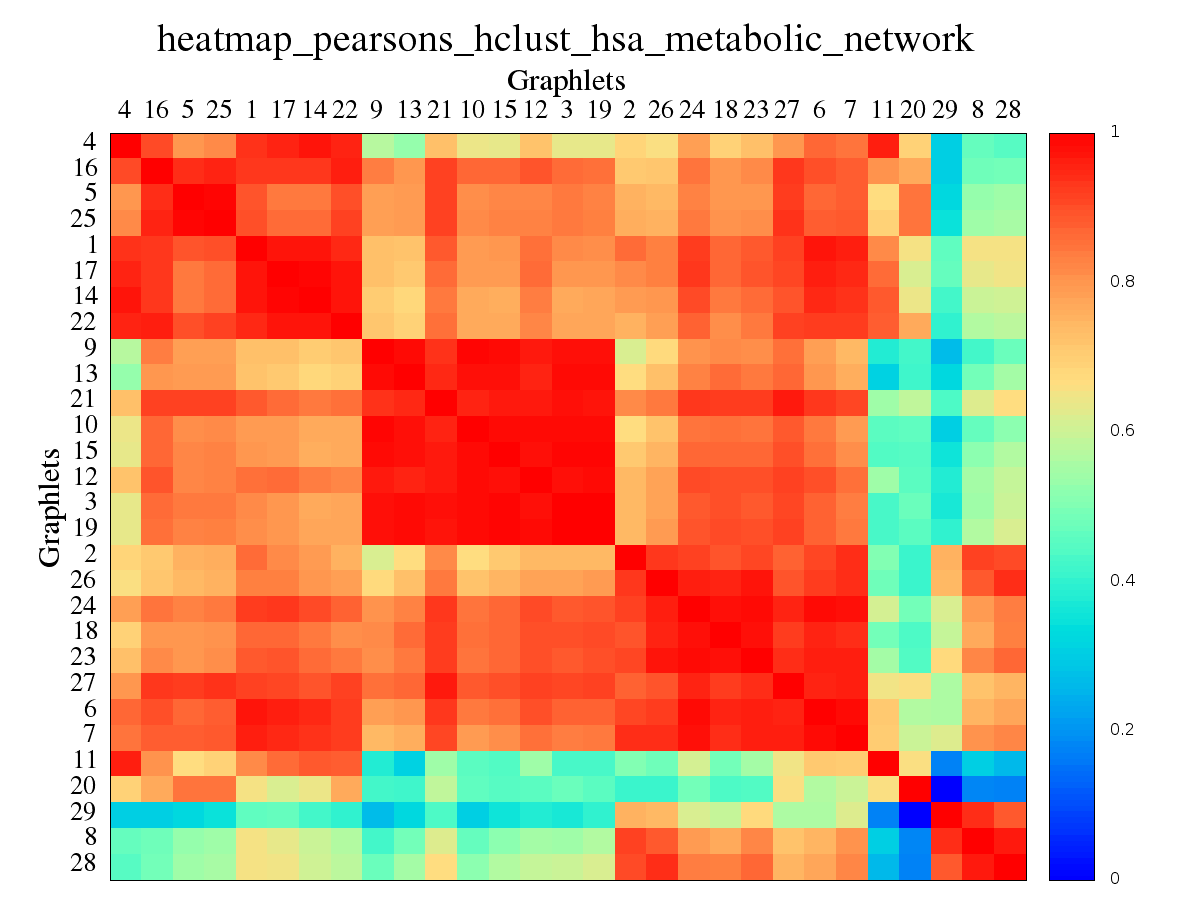
\includegraphics[scale=0.4]
{../code/final_results/hsa_metabolic_network/heatmap_pearsons_hclust_hsa_metabolic_network.png}
\caption{}
\label{fig:hsa_meta}
\end{figure}

For the HSA metabolic network, we can clearly see several clusters of graphlets that have been formed along the main diagonal. These are as follows:
\begin{enumerate}
 \item \textbf{Claw} cluster made of Graphlets {4,16,5,25,1,17,14,22}. These graphlets all have a C4 (claw - graphlet G4) as a subgraph.
 \item \textbf{Paths} cluster made of Graphlets {9,13,21,10,15,12,3,19}. These graphlets all have a P4 (path - graphlet G3) as a subgraph.
 \item \textbf{Triangles} cluster made of Graphlets {2,26,24,18,23,27,6,7}. These graphlets all have triangles (graphlet G2) as subgraphs
 \item \textbf{Cliques} cluster made of Graphlets {29,8,28}. These graphlets are cliques, with the exception of 28, which 
 is almost a clique as it is missing as edge. Note that the 3 node clique is missing because being a triangle, it is correlated more with the triangle group above.
 \end{enumerate}
 
Furthermore, we can also notice that graphlets from clusters 1,2,3 also have a high degree of inter-correlation, 
since they might contain claws, paths and triangles at the same time. This is not 
the case for group 4, which is made of cliques. The cliques only bear some 
correlation with the third cluster made of triangle-like graphlets, which is not surprising for the following reasons:
\begin{itemize}
 \item Cliques contian a lot of triangles
 \item Cliques do not contain claws C4 or paths P4, which miss several edges.
\end{itemize}

It should also be noted that graphlets 11 and 20 have been left outside, as they don't strongly correlate with any of the other groups. The cluster closest to these 2 grahlets is the claw cluster.

To sum up, we can see how the graphlets cluster together according to what basic shapes they contain.

\subsubsection*{CCA - Hsa metabolic Network (Compound-based)}

%\textcolor{red}{\textcolor{red}{"sig29"}}

\begin{tabular}{ c | l }
canonical correlation & 0.517688900136879\\
\hline
\textbf{"sig29"} & -0.34583422564784\\
\textbf{"sig2"} & -0.367846409747838\\
\textbf{"sig8"} & -0.374418098124076\\
\hline
"EC5" & -0.114222050692381\\
"EC2" & -0.126006303968814\\
"EC4" & -0.161439048762524\\
"EC1" & -0.161557005857164\\
"EC3" & -0.210568893756238\\
"EC6" & -0.406153663937205\\
\end{tabular}\\


There is some degree of correlation between the Graphlets and the EC numbers (0.517). All the cross-loadings from both the Graphlets and the EC numbers have the same sign, which suggests that they are positively correlated. Cliques 8, 2 and 29 have the highest magnitude in their weights, while EC6 (ligands) have the highest magnitude in the EC vector. 

EC6 refers to ligases, which are "enzymes that can catalyze the joining of two large molecules by forming a new chemical bond" (Wiki: http://en.wikipedia.org/wiki/Ligase). The reason why the magnitude of EC6 is quite high (0.4) compared to the other indicators is because the neighbourhood of the ligase compound is made of the two large molecules that have a lot of interactions and feedback loops between them. These interactions and feedback loops yield a high number of graphlets in the network topology.


\subsection*{Other metabolic networks}

We have analysed other metabolic networks that belong to the following organisms: C. elegans, D.melanogaster, E.coli, M.musculus, S.cerevisiae. For all these organisms, we have analysed both compound-based networks and also enzyme networks.

They results for the other compund-based networks confirm the correlation heatmaps and CCA results that were obtained for Homo Sapiens. Average CCA correlation is around 0.5, EC6 has the highest magnitude at around 0.4 and cliques 2,8,29 are usually the most correlated with it (~ 0.35).

However, the enzyme networks display a much lower CCA correlation (around 0.25). This is the case for all the organisms, including humans. The Graphlet signatures have very low signatures, while EC numbers don't have magnitudes above 0.22.

\subsubsection*{Example - CCA result for E.Coli - Enzyme-based Metabolic network}


\begin{tabular}{ c | l }
canonical correlation &  0.251508972397617\\
\hline
"sig25" & -0.0151119270013791\\
"sig5" & -0.0197252221535908\\
"sig20" & -0.0293681175027652\\
\hline
"EC1" & 0.159458849722403\\
"EC6" & 0.12180017345131\\
"EC3" & 0.0537111323926065\\
"EC4" & 9.93665948890473e-05\\
"EC5" & -0.0443838552104944\\
"EC2" & -0.21807362156073\\
\end{tabular}\\

\section*{PPI networks}
\subsection*{Human PPI}


\begin{figure}[H]
  \centering
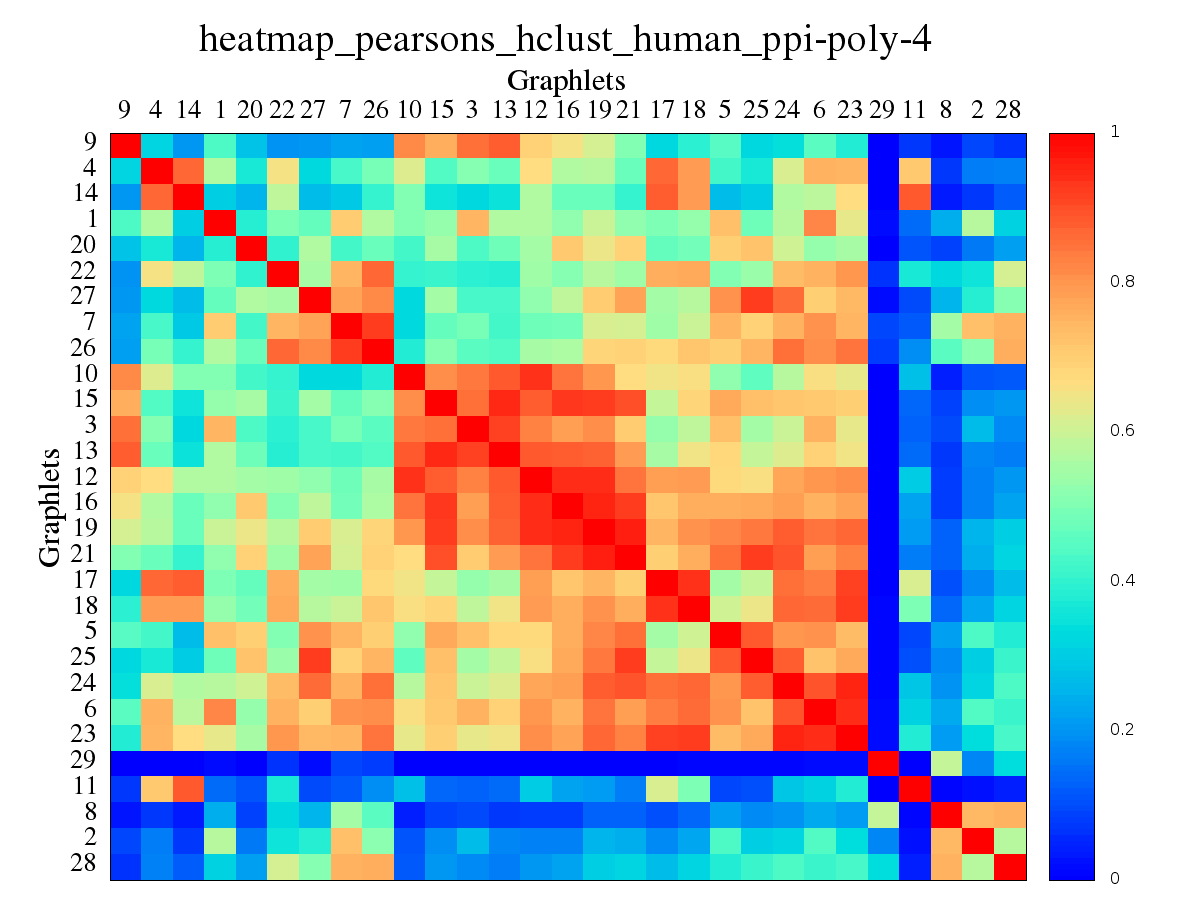
\includegraphics[scale=0.4]
{../code/final_results/human_ppi/heatmap_pearsons_hclust_human_ppi-poly-4.png}
\caption{}
\label{fig:human_ppi}
\end{figure}

The above figure represents the Pearsons's correlation heatmap for the Human PPI 
network. As opposed to the Metabolic network, the clusters obtained are much less 
noticeable. The cluster that seems most proeminent is made of Graphlets 10,15,3,13,12,16,19 and 21.
These graphlets all contain a P4 (path on 4 nodes, graphlet G3). 
This time, it also seems that the cliques are uncorrelated.

The lack of graphlet correlations in the Human PPI is something that we cannot 
explain at the current time. Further research needs to be done into this area. 


\subsubsection{Human PPI CCA}

\begin{tabular}{ c | l }
canonical correlation &  0.155502366337325\\
\hline
"sig1" & -0.0681076890184487\\
\textbf{"sig8"} & -0.071701548908936\\
\textbf{"sig29"} & -0.0721921026141832\\
\textbf{"sig2"} & -0.0816038161136185\\
\hline
"RNA.metabolism" & -0.065515997126898\\
"death" & -0.130453937016065\\
\end{tabular}\\



As it can be noticed the correlation is really low, suggesting that the number graphlet signatures doesn't reflect the annotations of the proteins. However, the CCA results for yeast look more promising (see next subsection)

\subsection*{The 18 experiments}

We performed CCA on 6 different human ppi networks with one annotation file and also on 6 yeast networks using 2 annotation files. The networks were as follows:

\begin{itemize}
 \item Human - one annotation file (14) -- 6 experiments in total
 \begin{enumerate}
    \item human HI 2012 preliminary
    \item human i2d full
    \item human i2d hc
    \item human ppi 56k
    \item biogrid human ppi noUBC full (removed the ubiquitous protein)
    \item biogrid human ppi hc
  \end{enumerate}
 \item Yeast - two annotation files: boone (14) and merin (13) -- 6x2 = 12 experiments in total
  \begin{enumerate}
    \item yeast apms collins
    \item yeast biogrid genetic
    \item yeast lc
    \item yeast y2h union yu ito uetz
    \item biogrid yeast ppi noYLL039C full (removed the ubiquitous protein)
    \item biogrid yeast ppi hc
  \end{enumerate}
\end{itemize}

The best results have been obtained for the following yeast networks, for both annotation files:
  \begin{enumerate}
    \item yeast apms collins 
    \item yeast biogrid genetic (correlation of 0.35 with boone)
    \item biogrid yeast ppi noYLL039C full (removed the ubiquitous protein)
    \item biogrid yeast ppi hc
  \end{enumerate}

They have an average overall CCA correlation of 0.5 (apart from \emph{yeast biogrid genetic}). On the graphlet side, the highest correlations are usually with cliques 2,8 and 29 (correlation values ~ 0.45-0.5). On the annotation side, the highest correlations are with translation (~ corr. value 0.5) (\emph{yeast apms collins} and \emph{biogrid yeast ppi noYLL039C full}), transcription (mainly \emph{biogrid yeast ppi hc}). Therefore, we can state that the proteins that are involved in translation or transcription are more likely to have a neighbourhood rich in graphlets, especially cliques.

The other combinations of networks and annotation files have yielded much poorer correlation results (only aprox 0.2). One of the reason for this might be because of the high noise of the data that is prevalent in PPI networks.

\subsubsection{Selected CCA Results}


\textbf{6: Yeast Colling apms - boone}\\

\begin{tabular}{ c | l }
canonical correlation &  0.530126834561433\\
\hline
"sig9" & -0.212189480521127\\
"sig10" & -0.23169736846479\\
... & ...\\
"sig7" & -0.454313584962548\\
\textbf{"sig29"} & -0.46430615776707\\
\textbf{"sig8"} & -0.479142491460243\\
\textbf{"sig2"} & -0.499532936369011\\
\hline
... & ...\\
"RNA.processing" & -0.0475609645756522\\
"Ribosome.translation" & -0.508987082686986\\
\end{tabular}\\\\\\

\textbf{10: Biogrid Yeast PPI noYLL039C full - boone}\\

\begin{tabular}{ c | l }
canonical correlation &  0.45880430741723\\
\hline
"sig11" & -0.0335008490033594\\
"sig14" & -0.0391537348322753\\
"sig10" & -0.0409595646198318\\
... & ...\\
"sig7" & -0.275508344217967\\
"sig28" & -0.289739702115225\\
\textbf{"sig29"} & -0.299368501765292\\
\textbf{"sig8"} & -0.324296804477194\\
\textbf{"sig2"} & -0.345230081760038\\
\hline
... & ...\\
"Chromatin.transcription" & -0.0283716381202604\\
"RNA.processing" & -0.240026232630838\\
"Ribosome.translation" & -0.352812642444517\\
\end{tabular}\\

\textbf{17: Biogrid Yeast ppi hc - merin}\\

\begin{tabular}{ c | l }
canonical correlation &  0.424493771565584\\
\hline
"sig11" & 0.00615470207634573\\
"sig4" & 0.00504623777854404\\
"sig14" & 0.00442874775308286\\
... & ...\\
"sig28" & -0.10302660841484\\
\textbf{"sig29"} & -0.11273512738831\\
"sig7" & -0.139579432212895\\
\textbf{"sig8"} & -0.165033816607569\\
\textbf{"sig2"} & -0.223518564656672\\
\hline
"X.M." & 0.0999257313876536\\
"X.A." & 0.0719525568889254\\
... & ...\\
"X.P." & 0.0036170242868089\\
"X.B." & -0.080911133899033\\
"X.T." (transcription) & -0.407239925520341\\
\end{tabular}\\\\

Von merin encoding:
\begin{itemize}
 \item E - energy production
 \item G - amino acid metabolism
 \item M - other metabolism
 \item P - translation
 \item T - transcription
 \item B - transcriptional control
 \item F - protein fate
 \item O - cellular organization
 \item A - transport and sensing
 \item R - stress and defense
 \item D - genome maintenance
 \item C - cellular fate / organization
 \item U - uncharacterized
\end{itemize}



\section*{Trade network}

\begin{figure}[H]
  \centering
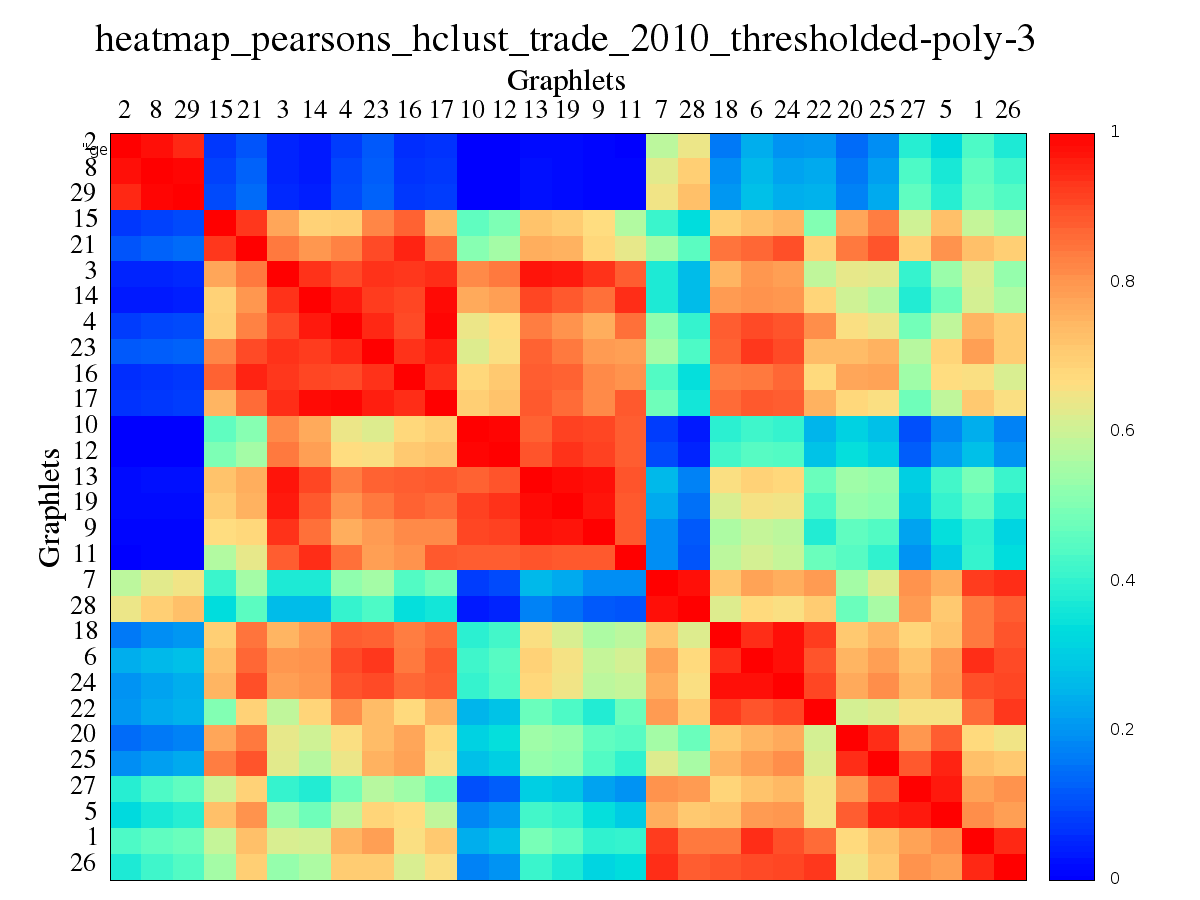
\includegraphics[scale=0.4]
{../code/final_results/trade_2010_thresholded/heatmap_pearsons_hclust_trade_2010_thresholded-poly-3.png}
\caption{}
\label{fig:trade}
\end{figure}

In the trade network, we can observe several clusters of graphlets that ahave been formed along the diagonal:
\begin{itemize}
 \item Cliques cluster made of graphlets 2,8,29. If a country has a lot of cliques in its neighbourhood, then it is part of a densely connected group of countries. 
 \item A cluster that is made of graphlets 15,21,3,14,4,23,16,17,10,12,13,19,9 
 and 11 which can be split into 2 further sub-clusters: 
    \begin{itemize}
     \item P4 cluster made of graphlets 15,21,3,14,4,23,16,17. These are all 
     graphlets that contain a P4 (path on 4 nodes, graphlet G3). 
     \item Claw cluster made of 10,12,13,19,9,11. These graphlets all contain C3 ( claw on 3 nodes, graphlet G4)
    \end{itemize}
\end{itemize}

\textbf{It should be noted that the diameter of the trade network is really small (aprox 5). This means that nodes will share a large proportion of their neighbourhood, especially hub nodes. In order to fix this issue, we have tried to threshold the economic networks at a level lower than 85\% in order to remove some of the edges and thus yield a higher diameter. However, this has not resulted in a lower diameter (it stayed constant at around 5), which meant that our metric might not be suitable for analysing this type of networks.}

\section*{Trade network over the years}

\subsection*{1962 to 1972}

\begin{figure}[H]
  \centering
  \label{fig:asafa}
  
  \subfloat{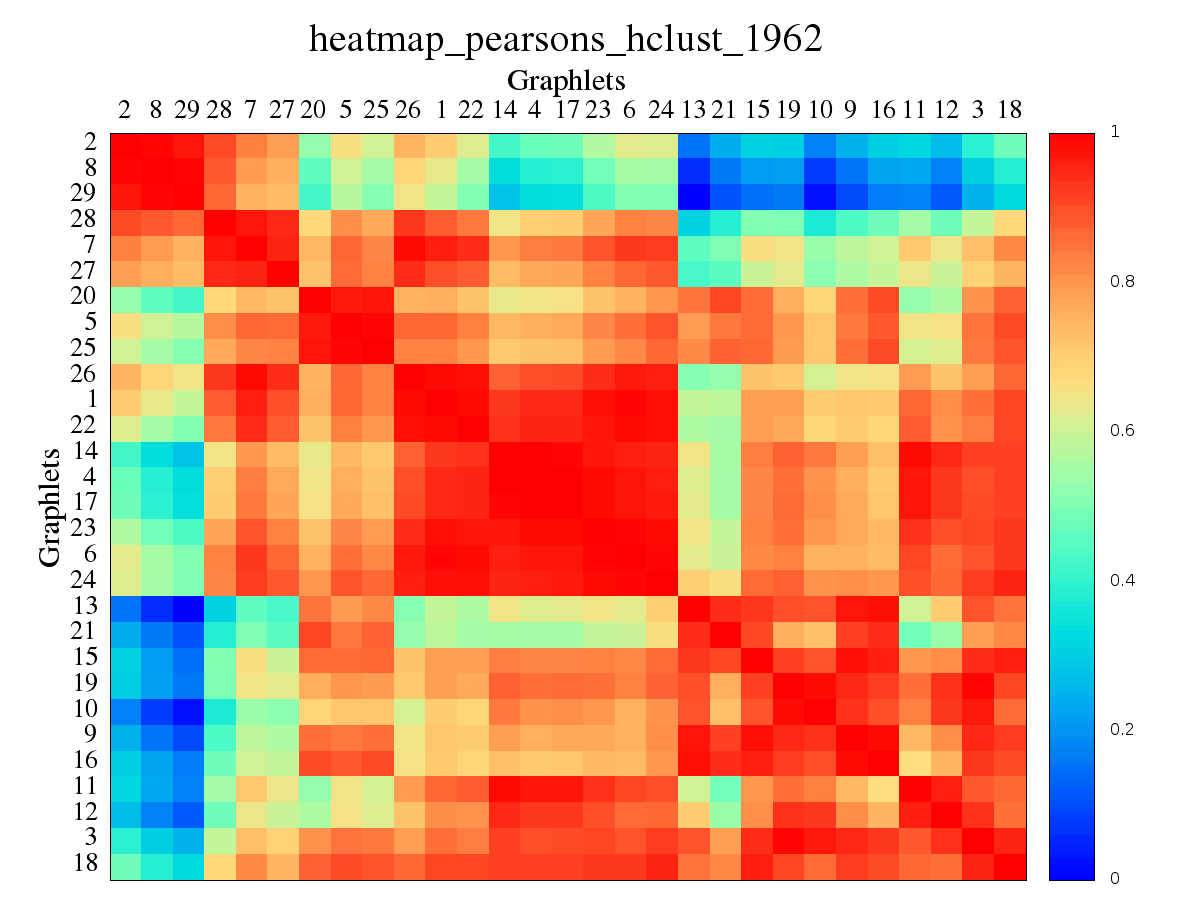
\includegraphics[width=70mm]{../code/final_results/all_trade_thresh/heatmap_pearsons_hclust_1962.png}}
  \subfloat{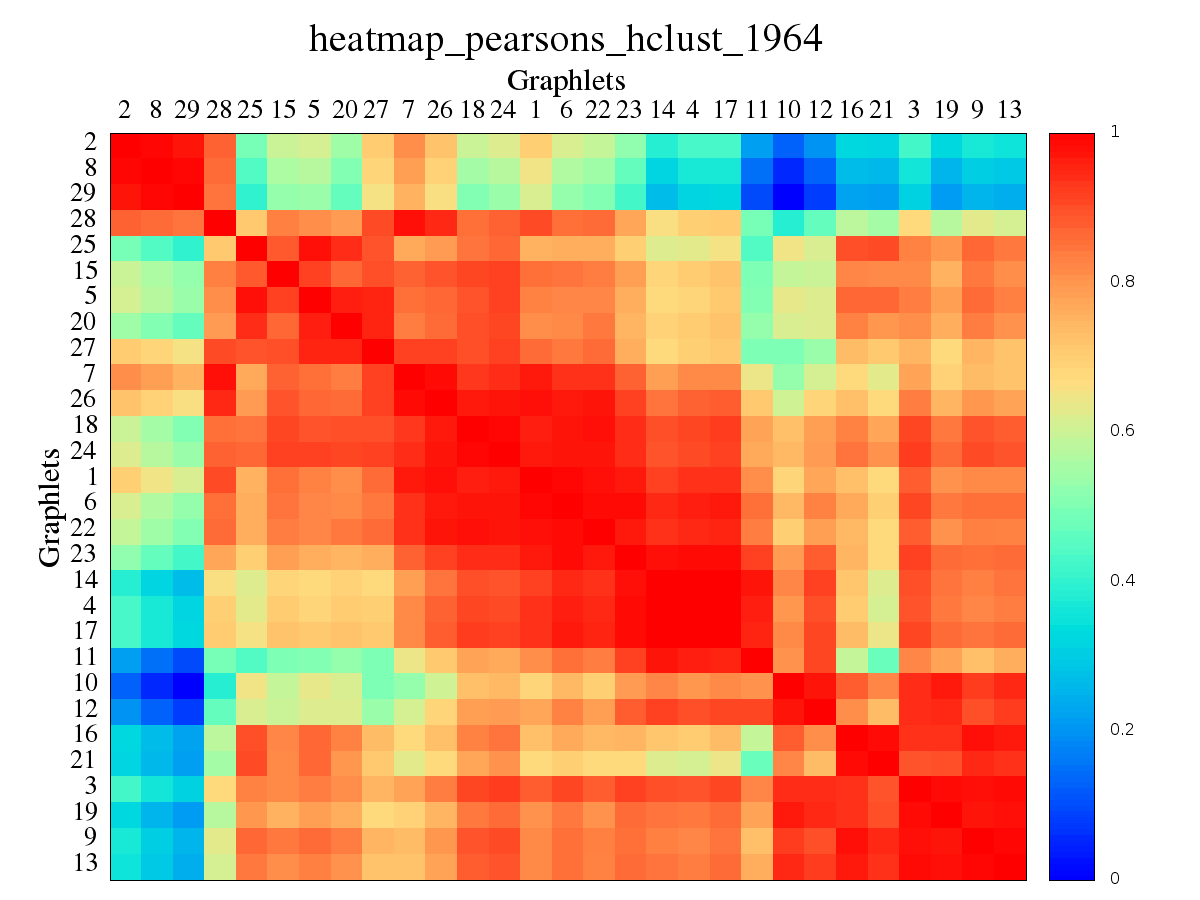
\includegraphics[width=70mm]{../code/final_results/all_trade_thresh/heatmap_pearsons_hclust_1964.png}}
  \\
  \subfloat{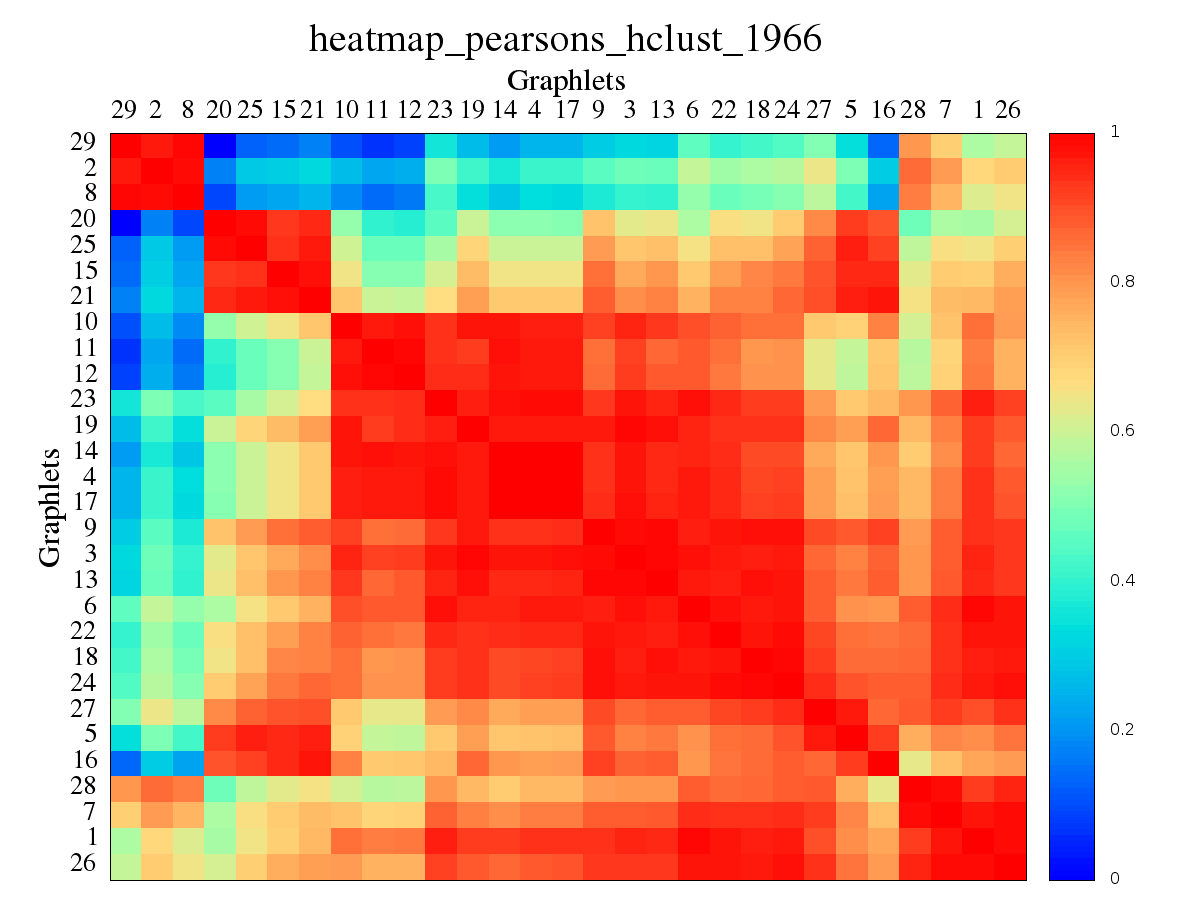
\includegraphics[width=70mm]{../code/final_results/all_trade_thresh/heatmap_pearsons_hclust_1966.png}}
  \subfloat{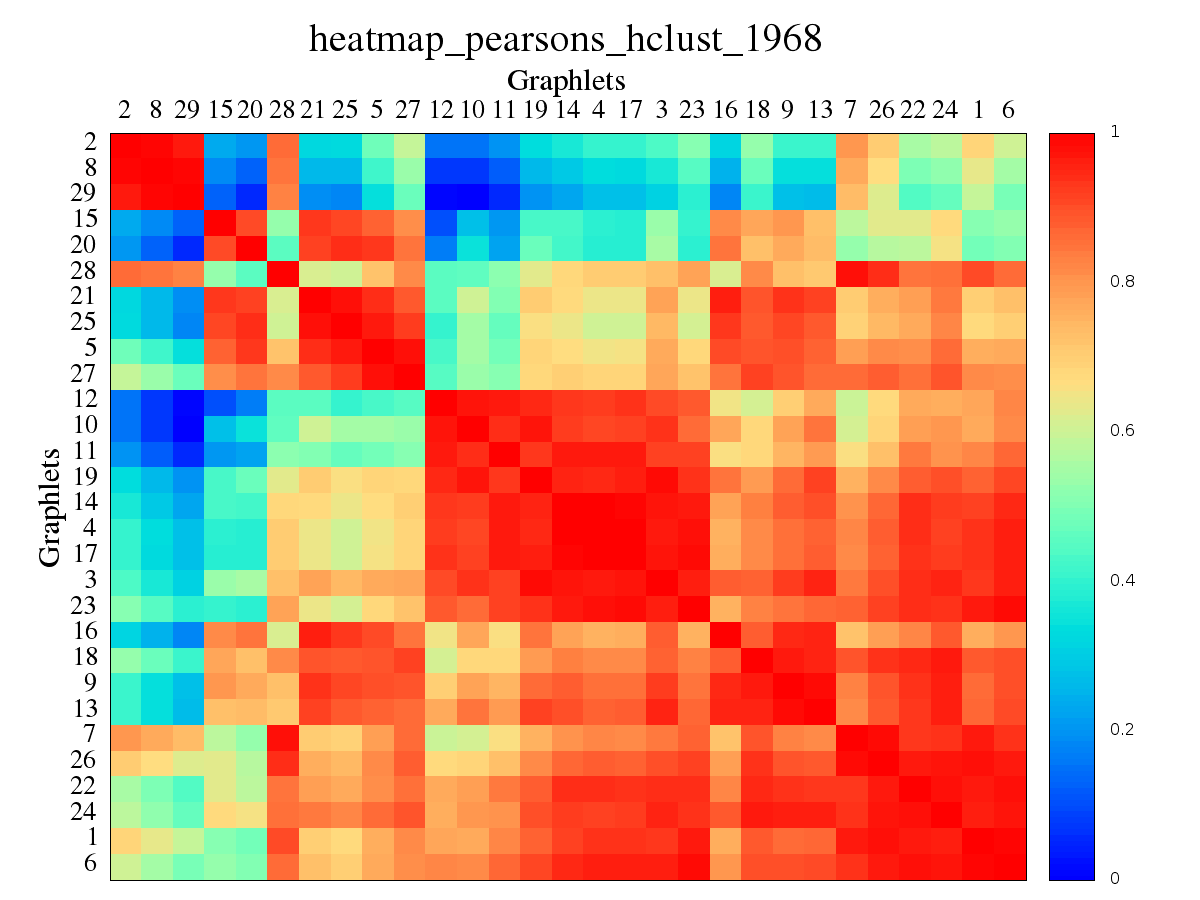
\includegraphics[width=70mm]{../code/final_results/all_trade_thresh/heatmap_pearsons_hclust_1968.png}}
  \\
  \subfloat{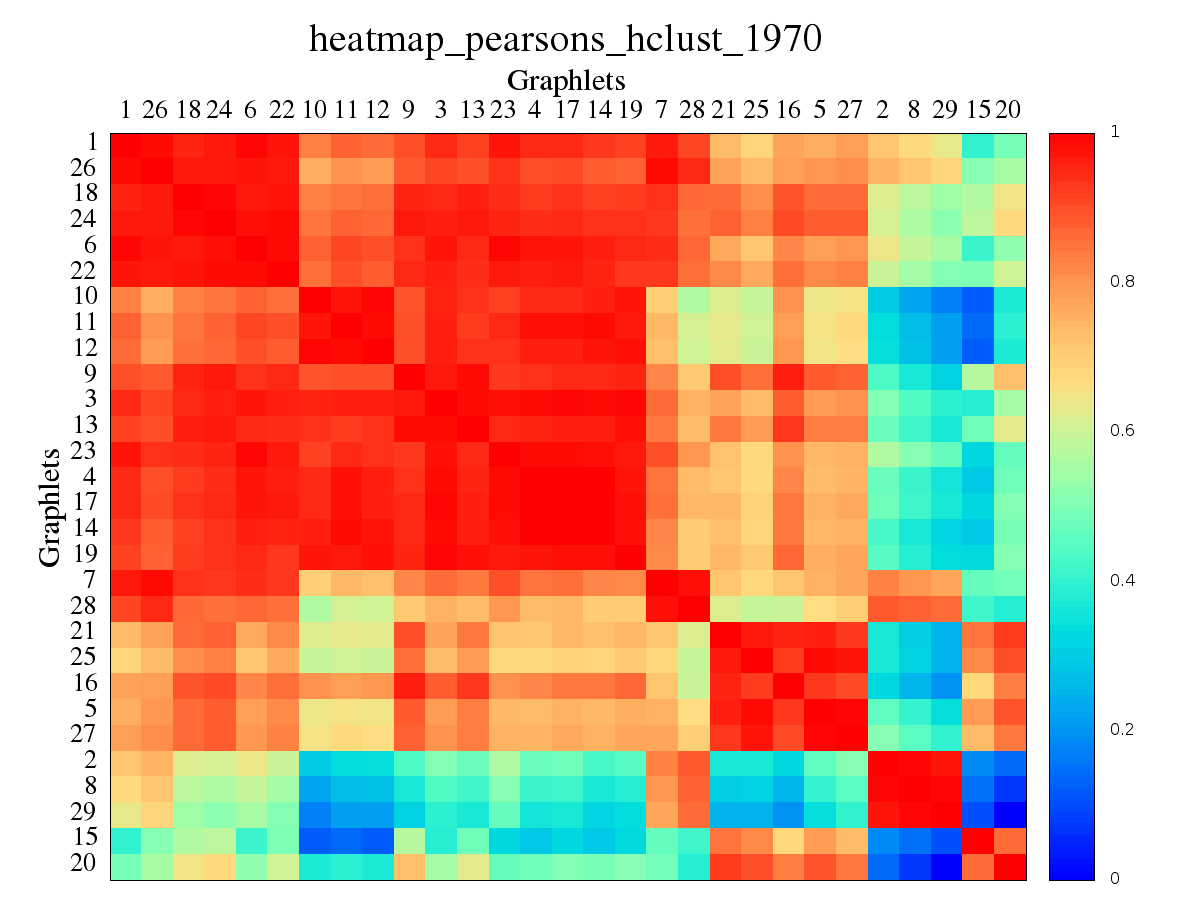
\includegraphics[width=70mm]{../code/final_results/all_trade_thresh/heatmap_pearsons_hclust_1970.png}}
  \subfloat{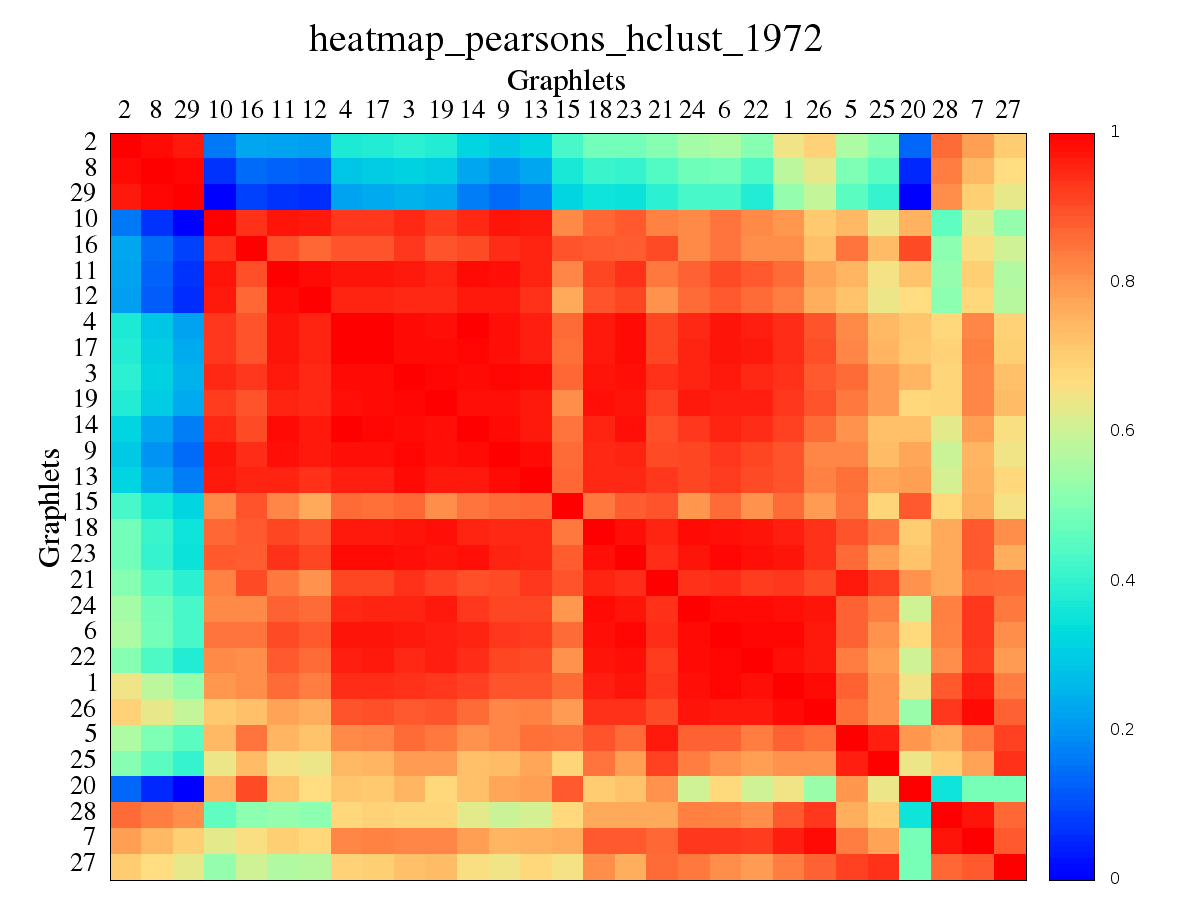
\includegraphics[width=70mm]{../code/final_results/all_trade_thresh/heatmap_pearsons_hclust_1972.png}}

\end{figure}

The first thing we notice is that the cliques 2,8 and 29 cluster together in each 
of the years analysed. In most of the years (apart from 1972) we also observe a 
cluster containing Graphlets that are made of cycles of length 4 (graphlet G5), 
with proeminent graphlets including 5, 20, 21 and 25. 

Another trend we notice is that the graphlets become more and more correlated 
(this will be even more obvious in the second batch of years 1974-1984). This 
might be an effect of globalization, as countries become more and more connected 
and the diameter of the trade network gets smaller. This in turn causes the 
countries to have share a higher proportion of the neighbourhood, which yields 
a higher graphlet correlation.




\subsection*{1974 to 1984}

\begin{figure}[H]
  \centering
  \label{fig:asafa}
  
  \subfloat{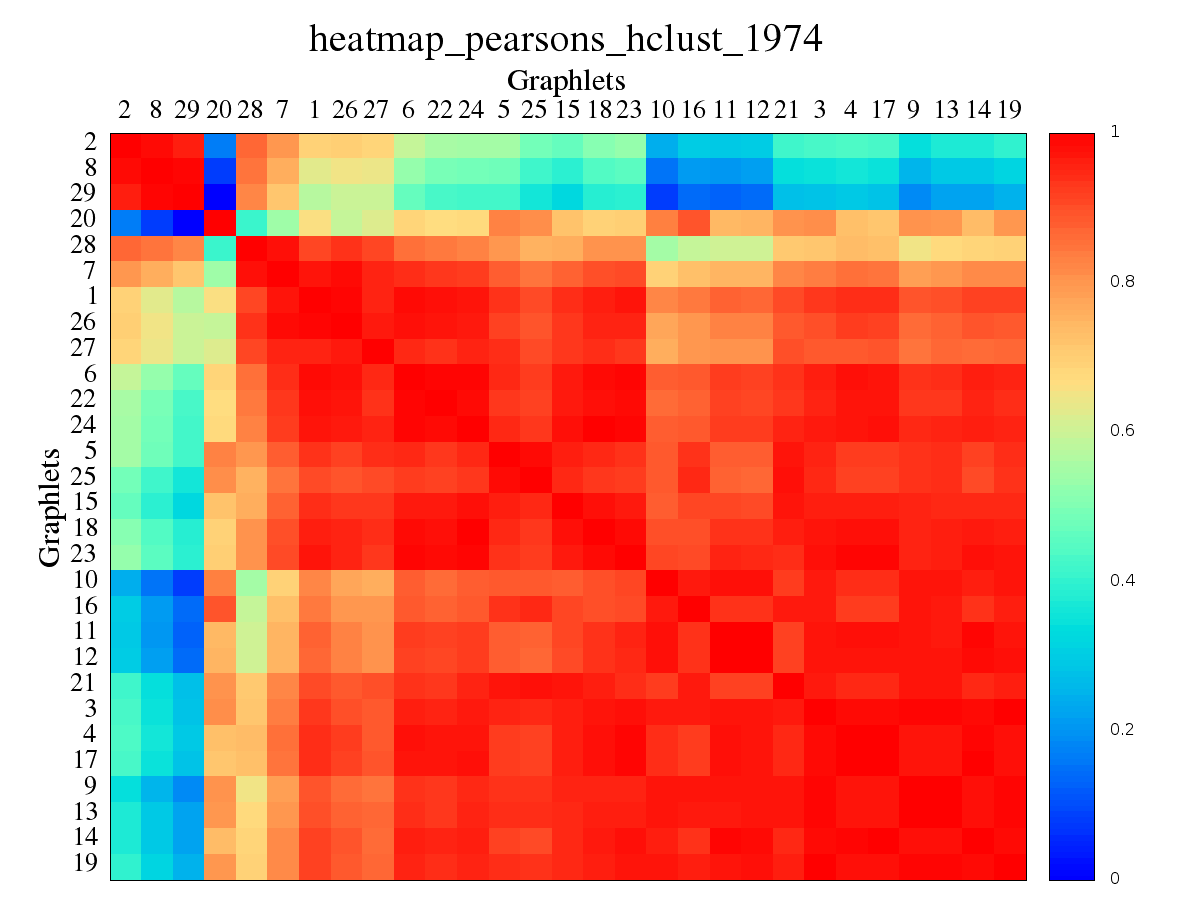
\includegraphics[width=70mm]{../code/final_results/all_trade_thresh/heatmap_pearsons_hclust_1974.png}}
  \subfloat{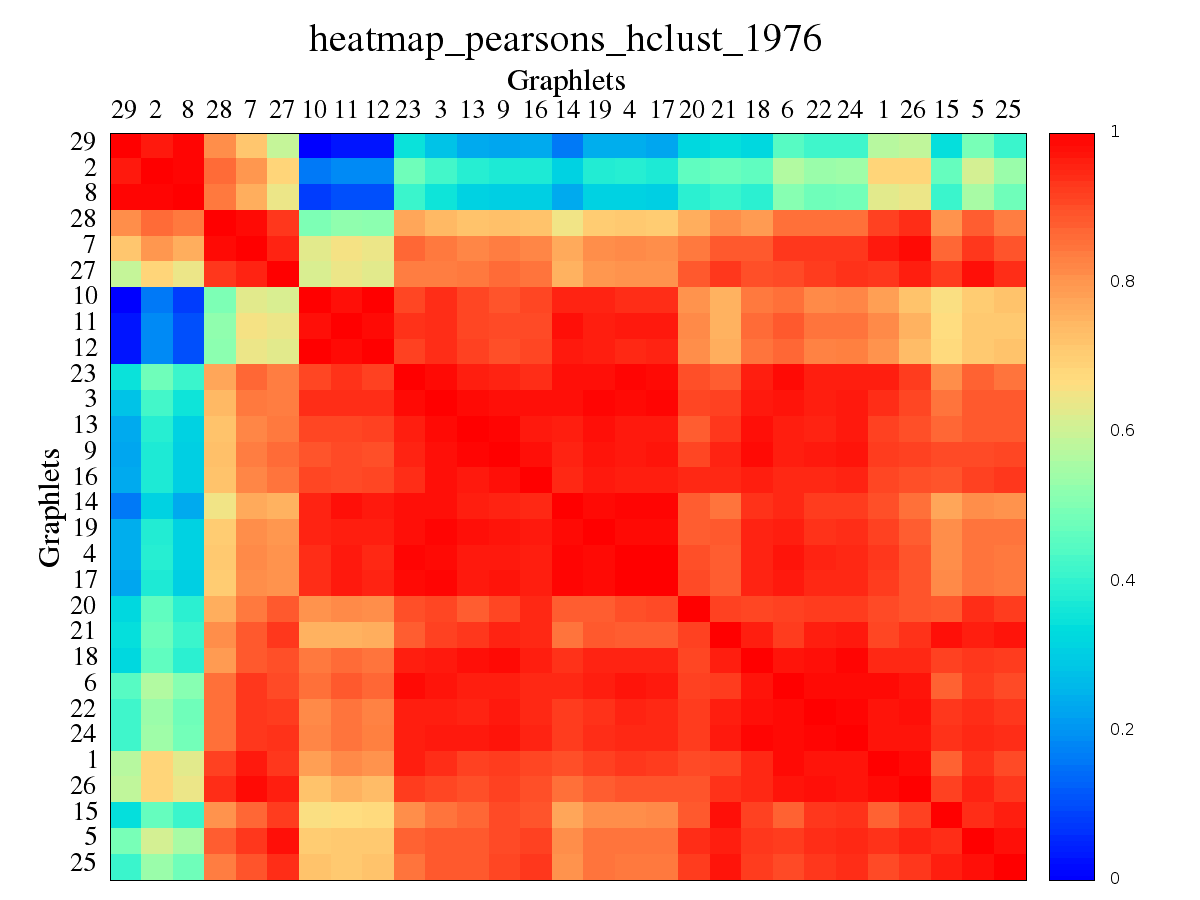
\includegraphics[width=70mm]{../code/final_results/all_trade_thresh/heatmap_pearsons_hclust_1976.png}}
  \\
  \subfloat{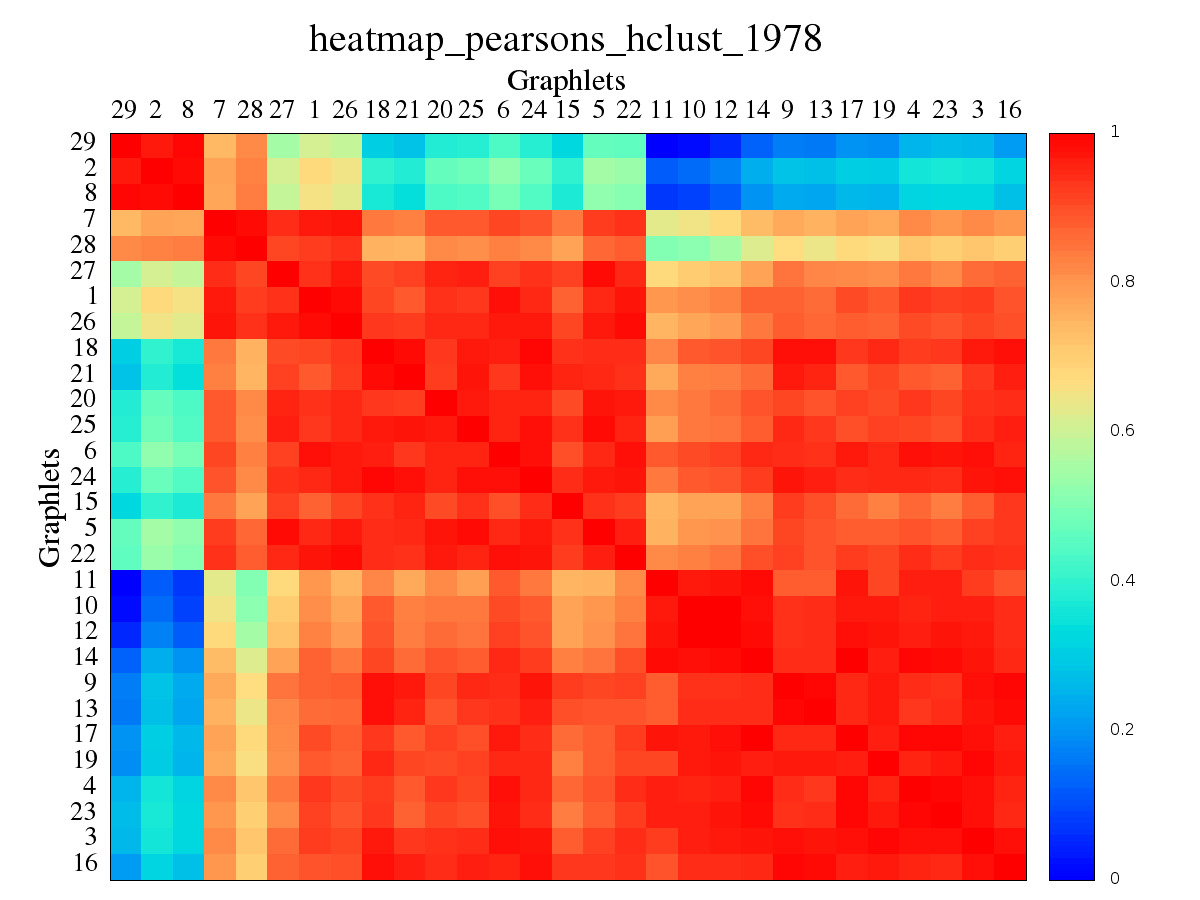
\includegraphics[width=70mm]{../code/final_results/all_trade_thresh/heatmap_pearsons_hclust_1978.png}}
  \subfloat{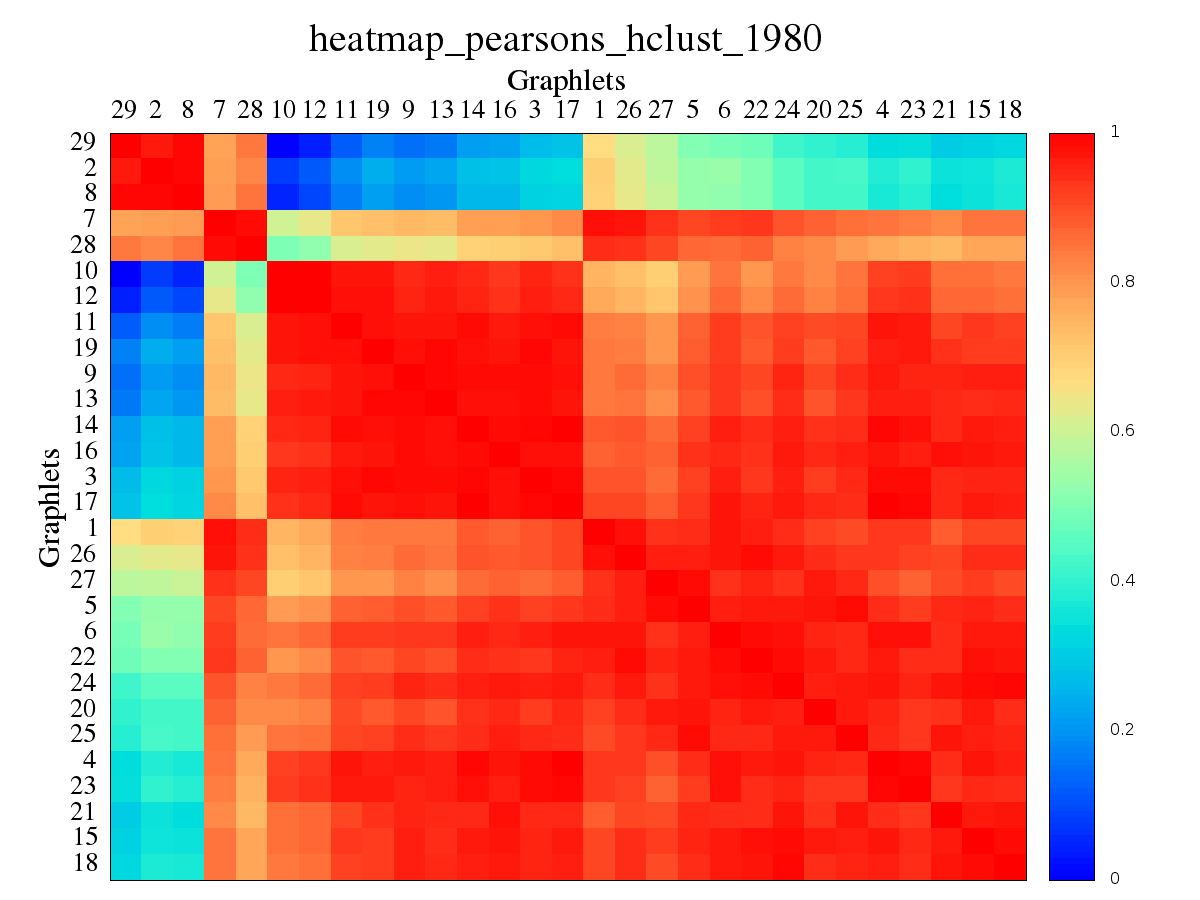
\includegraphics[width=70mm]{../code/final_results/all_trade_thresh/heatmap_pearsons_hclust_1980.png}}
  \\
  \subfloat{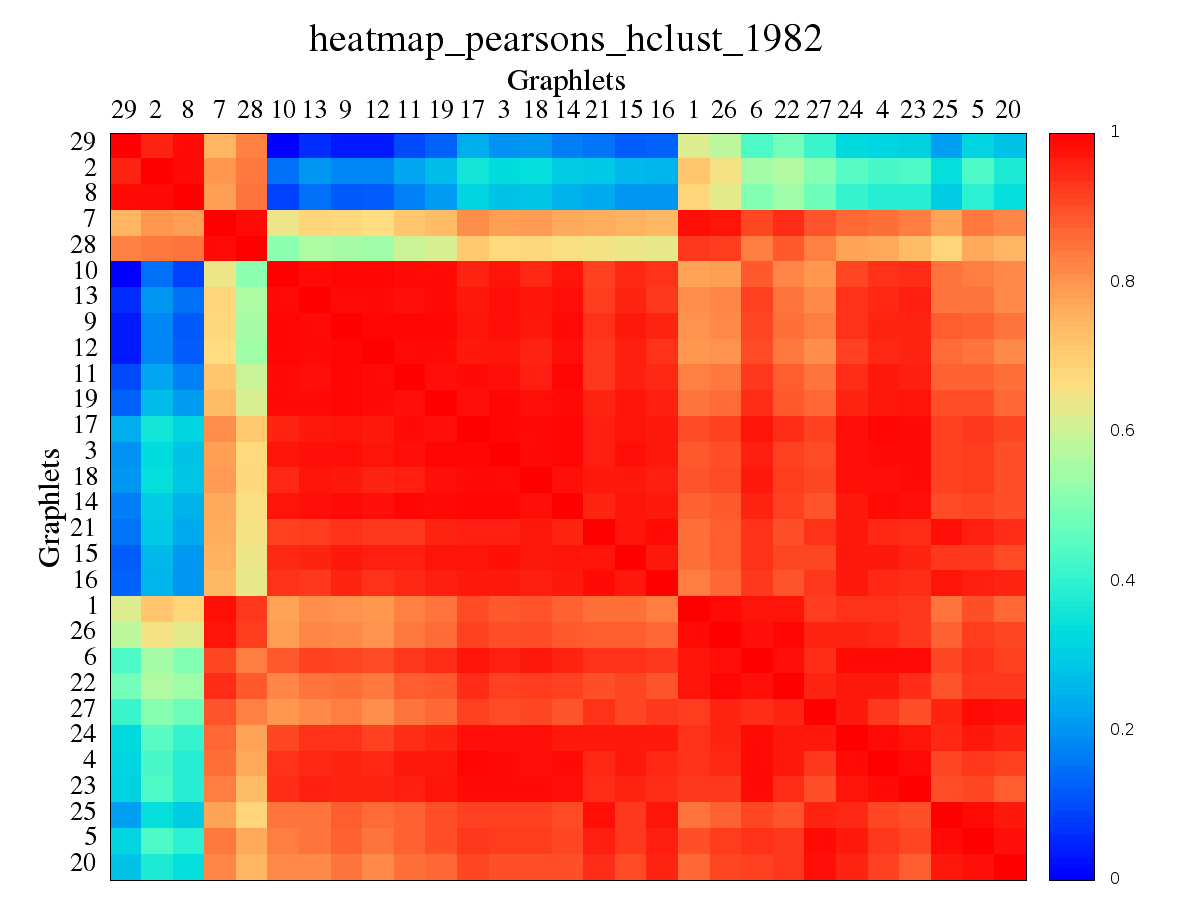
\includegraphics[width=70mm]{../code/final_results/all_trade_thresh/heatmap_pearsons_hclust_1982.png}}
  \subfloat{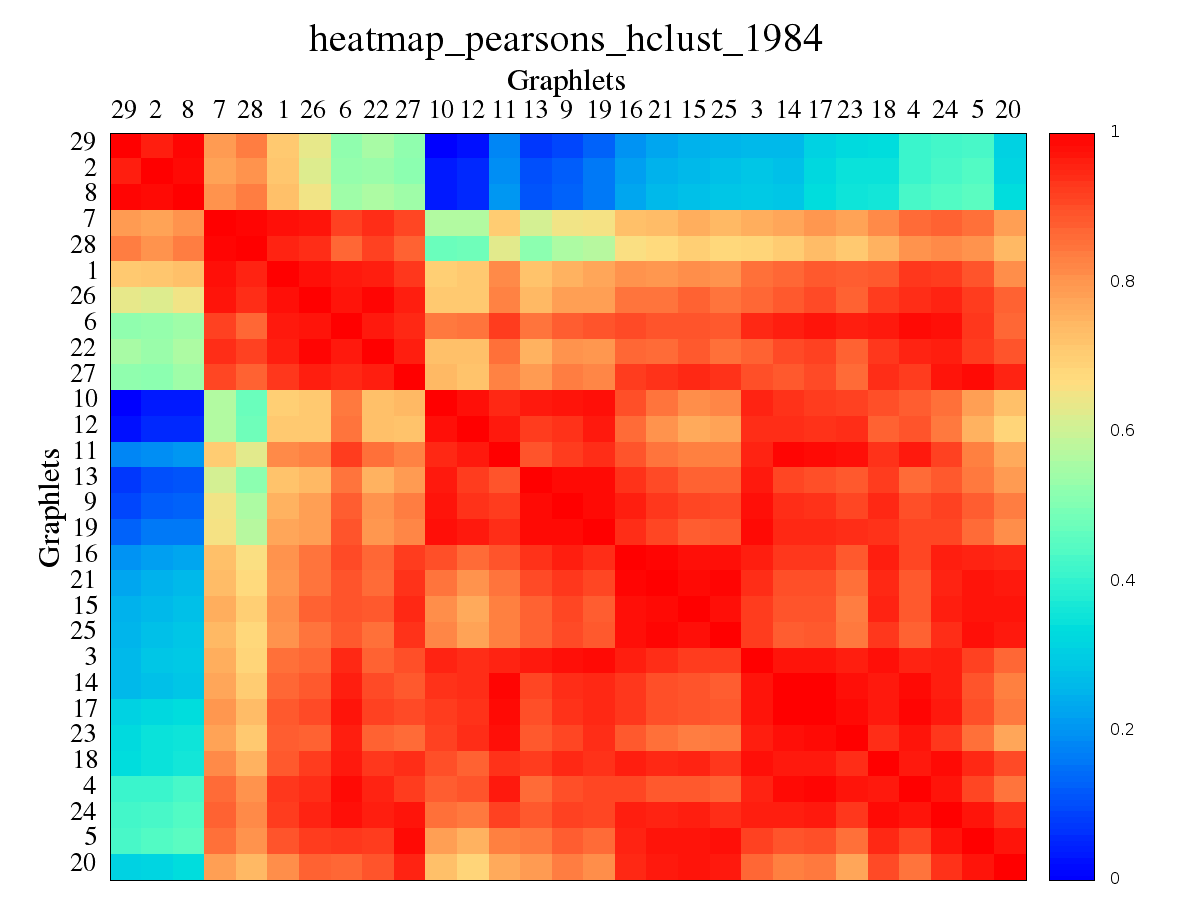
\includegraphics[width=70mm]{../code/final_results/all_trade_thresh/heatmap_pearsons_hclust_1984.png}}

\end{figure}

We also observe that the cliques 2,8 and 29 cluster together in every year 
that has been analysed in this period. In year 1980 we also observe  a cluster 
that is made of graphlets 10,12,11,19,9,13,14,16,3 and 17. All of these 
contain P4's (paths of length 4, graphlet G3). This cluster on P4 can also be 
observed in years 1976 and 1982, but the order in which graphlets appear is 
different, due to the clustering algorithm.

In year 1984, we can actually notice several small clusters on the diagonal. 
One cluster is made of graphlets 7, 28, 1, 26, 6, 22 and 27, which all have a 
P3 (path on 3 nodes, grahplet G1). However, cluster 10,12,11,13,9,19 is 
made of graphlets that don't seem to have a lot in common apart from P2's. 
Cluster 16,21,15 and 25 is mostly made of graphlets that have cycles of length 
4, apart from graphlet G15 which has a cycle of length 5.

On broad terms, we also notice that the graphlets become much more correlated 
in this period, as a result of globalisation. 

\subsection*{1986 to 1996}

\begin{figure}[H]
  \centering
  \label{fig:asafa}
  
  \subfloat{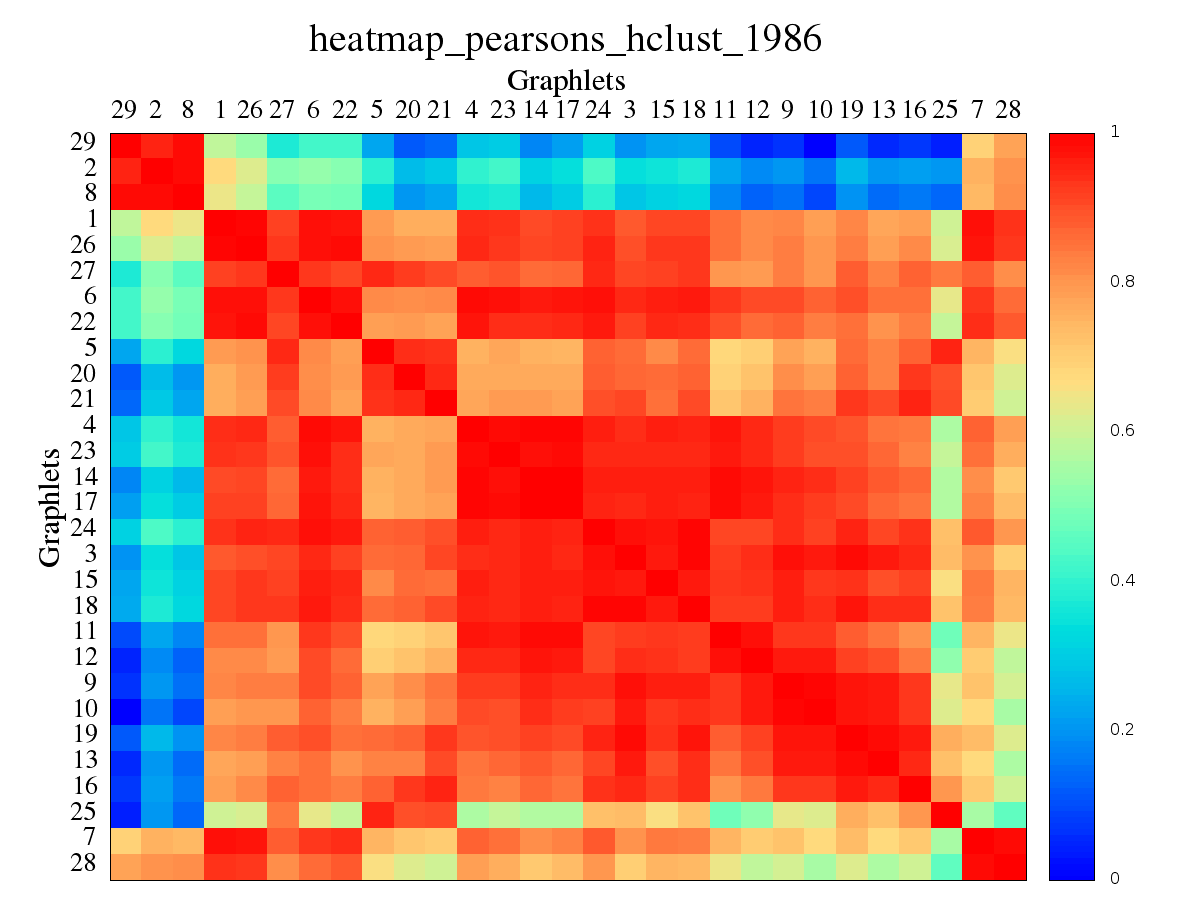
\includegraphics[width=70mm]{../code/final_results/all_trade_thresh/heatmap_pearsons_hclust_1986.png}}
  \subfloat{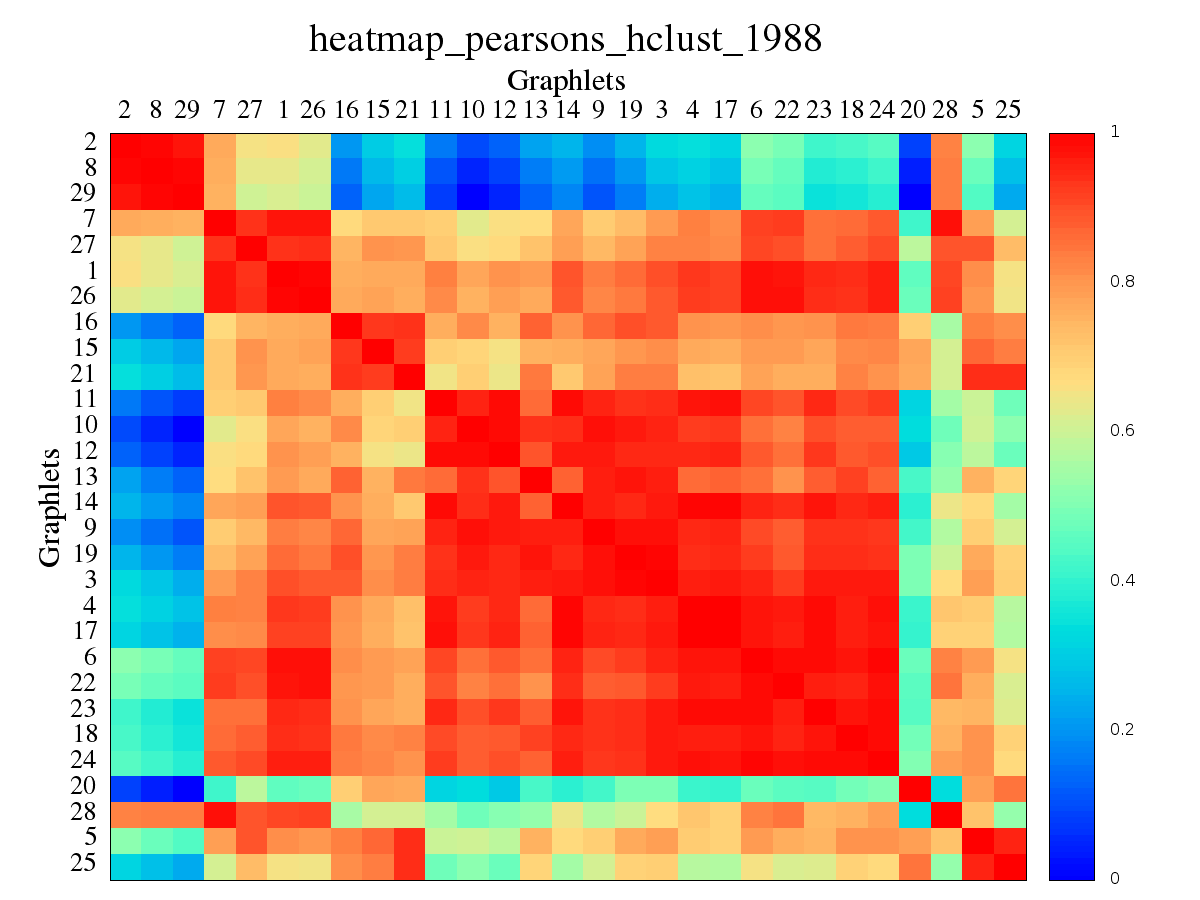
\includegraphics[width=70mm]{../code/final_results/all_trade_thresh/heatmap_pearsons_hclust_1988.png}}
  \\
  \subfloat{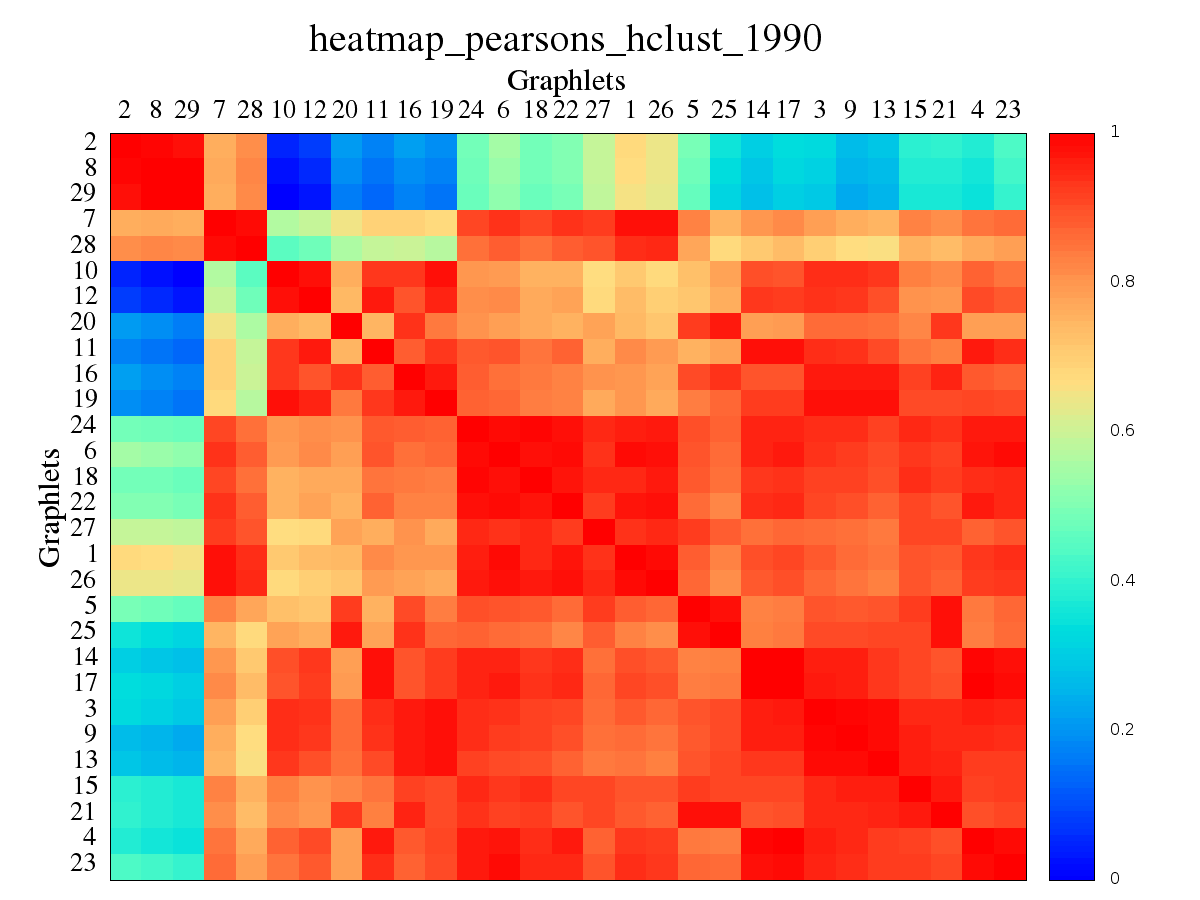
\includegraphics[width=70mm]{../code/final_results/all_trade_thresh/heatmap_pearsons_hclust_1990.png}}
  \subfloat{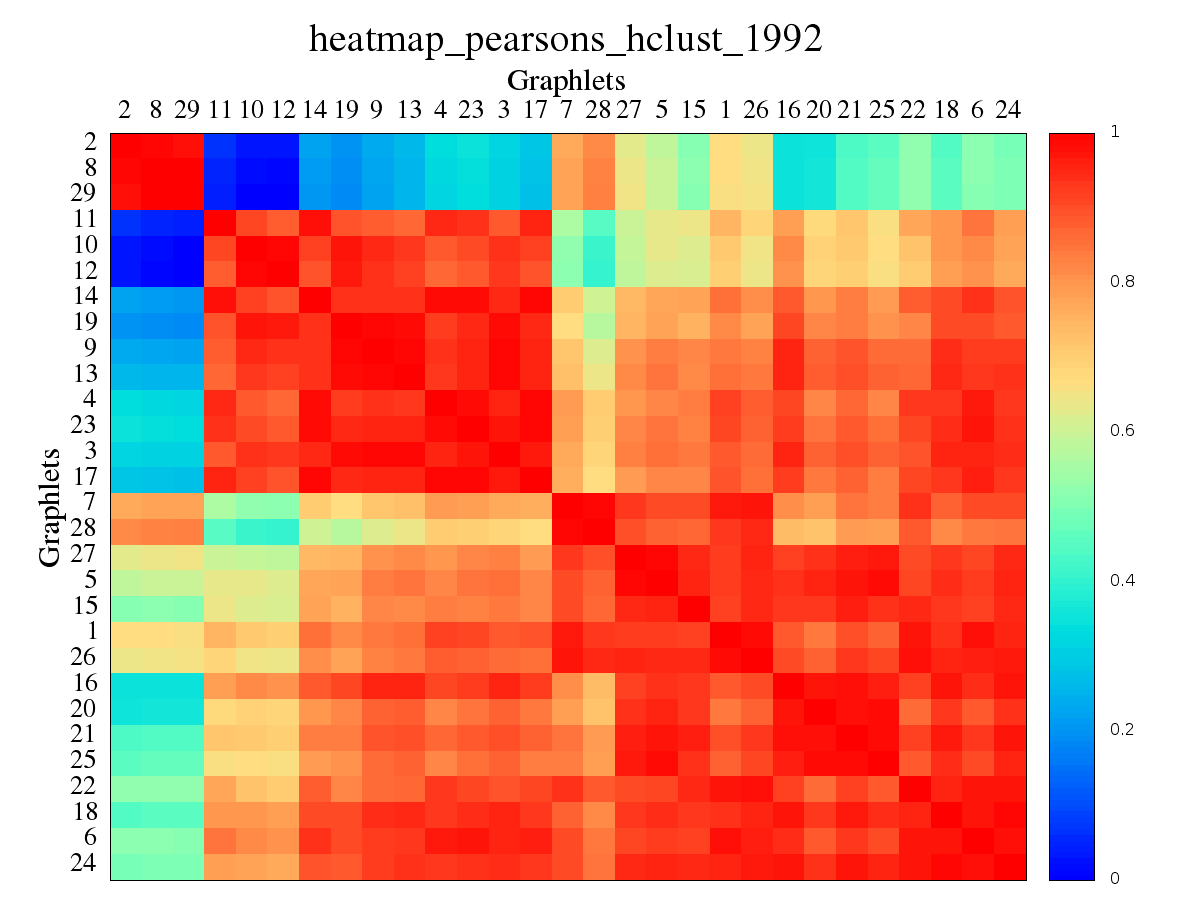
\includegraphics[width=70mm]{../code/final_results/all_trade_thresh/heatmap_pearsons_hclust_1992.png}}
  \\
  \subfloat{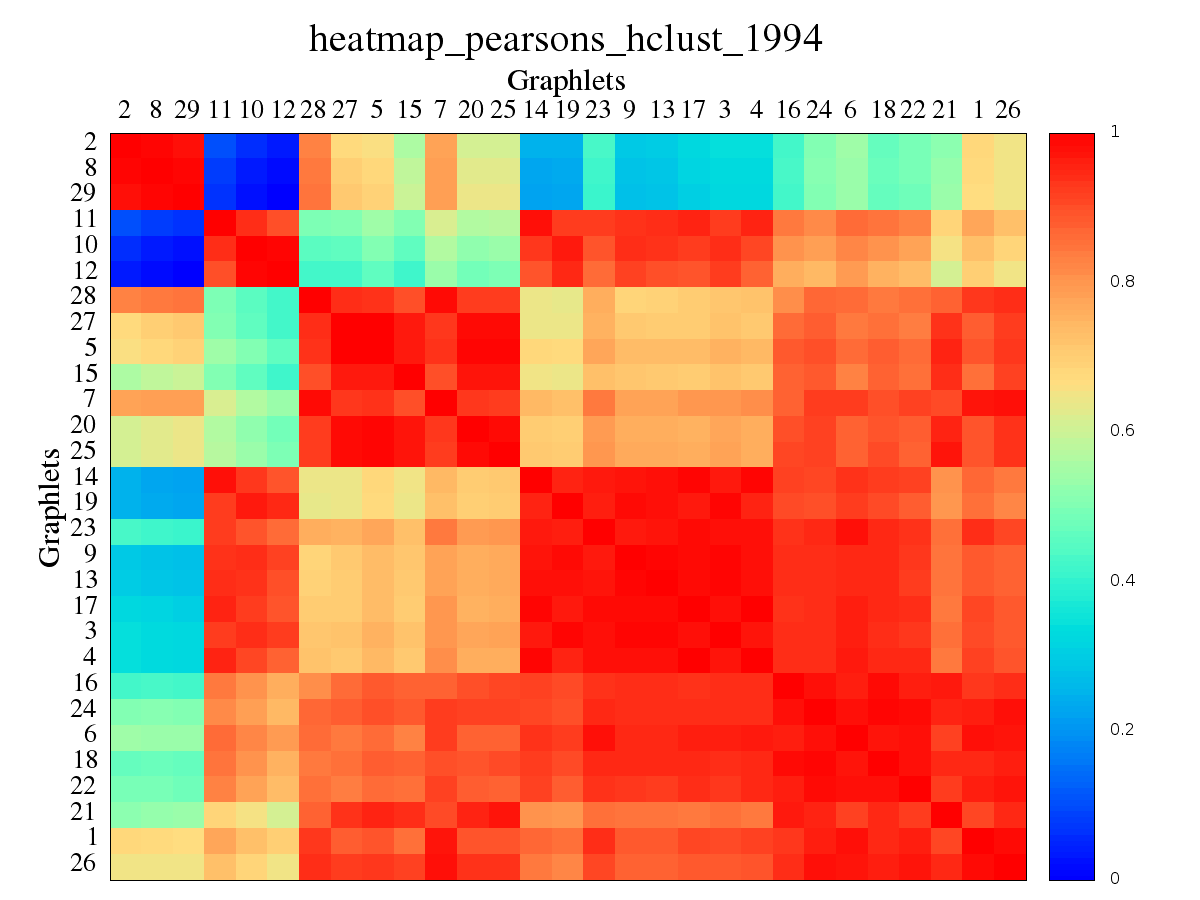
\includegraphics[width=70mm]{../code/final_results/all_trade_thresh/heatmap_pearsons_hclust_1994.png}}
  \subfloat{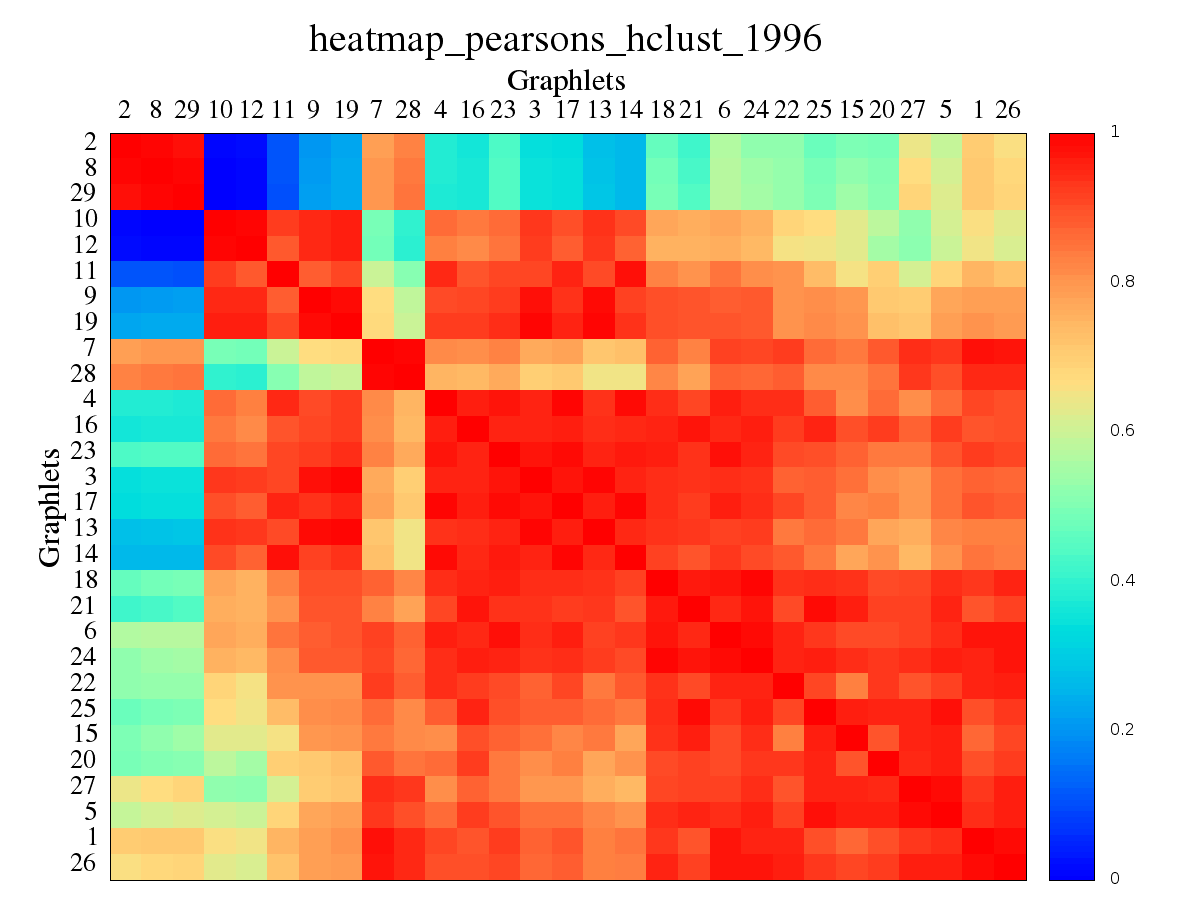
\includegraphics[width=70mm]{../code/final_results/all_trade_thresh/heatmap_pearsons_hclust_1996.png}}

\end{figure}



\appendix
% these do NOT count as part of the suggested page count
% This is probably a good place to explain the models in some detail for example


\subsection*{Trade 1980 - 2010 - CCA results}


\begin{tabular}{ c | l }
canonical correlation &  0.895952852603906\\
\hline
"OPENK" & 0.247451850129221\\
"BCA" & 0.200192036020745\\
"KG" & 0.174218020898056\\
"BCAperRGDPL" & 0.147747854581897\\
"KI" & 0.0599886767878585\\
"KC" & -0.0978003022187681\\
"XRAT" & -0.119986658349081\\
"KIxRGDPL" & -0.178691495415784\\
... & ...\\
"KIxRGDPLxPOP" & -0.725521757848721\\
"LE" & -0.758181971837348\\
"POP" & -0.766671415171843\\
\hline
"sig20" & -0.444543442451426\\
"sig15" & -0.575462152591753\\
"sig16" & -0.622031342349607\\
"sig25" & -0.637543533431093\\
... & ...\\
"sig3" & -0.783606882407559\\
"sig7" & -0.793649835514637\\
"sig6" & -0.803147167225324\\
\textbf{"sig2"} & -0.805688869837944\\
"sig1" & -0.823315620830077\\
\end{tabular}\\


CCA results clearly show that big and rich countries that have a high population and GDP per capita have a neighbourhood rich in Graphlets, while small and poor countries with account deficits have a sparser neighbourhood. The population of the country seems to be quite an important factor for determining whether it will have a neighbourhood rich in graphlets because of the following two reasons:
\begin{itemize}
 \item In the indicators vector, population has the weight with the highest magnitude: 0.766
 \item Most of the other indicators that have a high weight are obtained by mutiplying population with other indicators. It should be noted that this is the case also in Omer et al's paper "Revealing the hidden language" ...
\end{itemize}


\subsection*{Canonical correlation analysis on Economic Integration}

I have tried to analayse whether the level of \emph{Economic Integration} of a country is positively correlated with dense graphlets and negatively correlated with sparse graphlets. This is something to be expected, since when a country is part of a strong trading bloc, then it's neighbours have a higher probability of doing heavy trade with one another. This is because there is incentive for the country to trade more with the partners from the same bloc. This would in turn result in denser graphlets in the neighbourhood of that country. 

I have therefore annotated each country with a number (1-6) that measures the degree of economic integration:
\begin{itemize}
 \item 0 - no economic integration 
 \item 1 - Multilateral Free Trade Area (AFTA, CEFTA, CISFTA, COMESA, GAFTA, GCC
 \item 2 - Customs union (CAN, CUBKR, EAC, EUCU, MERCOSUR, SACU)
 \item 3 - Common market (EEA, EFTA, CES) 
 \item 4 - Customs and Monetary Union (CEMAC/franc, UEMOA/franc) 
 \item 5 - Economic union (CSME, EU) 
 \item 6 - Economic and monetary union (CSME/EC dollar, EU euro)
\end{itemize}


\begin{tabular}{ c | l }
canonical correlation &  0.618823452163313\\
p-value (asymptotic Wilks): & 0.0128012383082338\\
\hline
"Integration" & 0.618823452346073\\
\hline
\textbf{"sig29"} & 0.287035191288073\\
\textbf{"sig8"} & 0.283489421651237\\
\textbf{"sig2"} & 0.278615840865378\\
"sig22" & 0.26819674644438\\
"sig28" & 0.268059123234175\\
"sig7" & 0.260207030053052\\
"sig26" & 0.260112720674704\\
"sig18" & 0.246614831141233\\
"sig1" & 0.238368565474503\\
"sig24" & 0.231333551025451\\
"sig6" & 0.229690387810875\\
"sig4" & 0.220206855982917\\
"sig27" & 0.220129084450554\\
"sig17" & 0.210208580507573\\
"sig14" & 0.206306944610344\\
"sig23" & 0.204204021795578\\
"sig5" & 0.201486106029494\\
"sig20" & 0.193906989388751\\
"sig25" & 0.191223668928417\\
"sig21" & 0.190762668949242\\
"sig16" & 0.190257968164896\\
"sig11" & 0.183299329835195\\
"sig3"& 0.177301380839247\\
"sig15"& 0.168139476991408\\
"sig13"& 0.16763975453569\\
"sig19"& 0.160509773821264\\
"sig9" &0.150872182634174\\
"sig12"& 0.148861465107402\\
"sig10"& 0.146375591601729\\
\end{tabular}\\

\subsection*{Change over years}

\begin{figure}[H]
  \centering
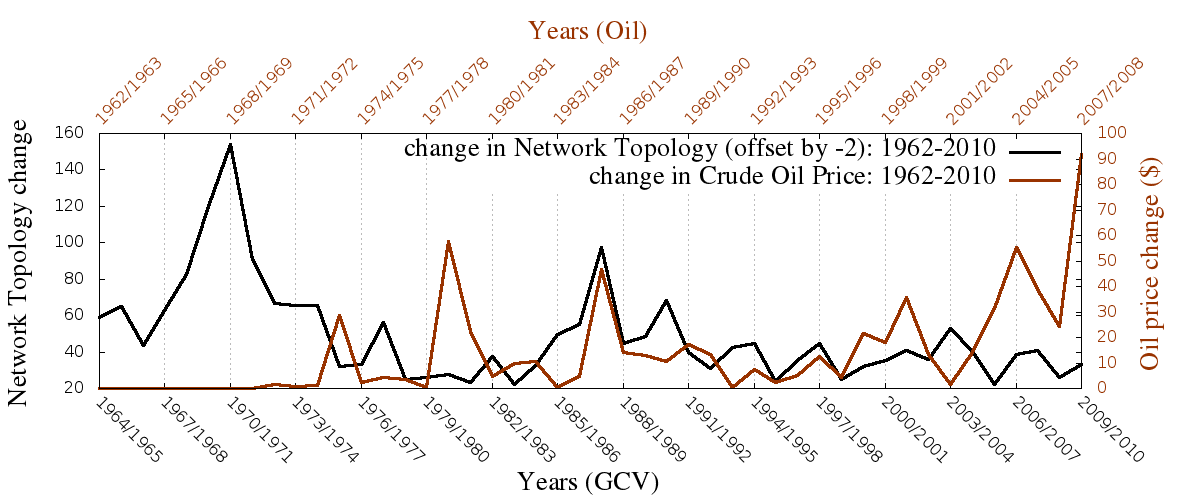
\includegraphics[scale=0.4]
{../code/final_results/all_trade_thresh/change_over_time.png}
\caption{}
\label{fig:hsa_meta}
\end{figure}

Important economic events that match the graph:
\begin{itemize}
 \item Black Monday of 1987
 \item OPEC oil crisis 1973 (although the peak in our graph occurs 3 years earlier)
 \item 1990's revolutions in Eastern Europe that mark a starting point of 
 increasing trade between Western Europe and Eastern Europe
 \item Arab Spring Revolts
\end{itemize}


\subsection*{Food and live animals - CCA results}


\begin{tabular}{ c | l }
canonical correlation &  0.954399648341325\\
\hline
"BCA" & 0.547689925367287\\
"BCAperRGDPL" & 0.500823424204372\\
"OPENK" & 0.243606879775848\\
"KI" & 0.209884267951759\\
... & ...\\
"KCxRGDPL" & -0.420546719870103\\
"KIxRGDPLxPOP" & -0.871656464696992\\
"LE" & -0.877434636132884\\
"POP" & -0.881642665100747\\
"KGxRGDPLxPOP" & -0.902330822089951\\
"RGDPLxPOP" & -0.911676654572702\\
"RGDPCHxPOP" & -0.911684561314991\\
"RGDPL2xPOP" & -0.911764842878327\\
"KCxRGDPLxPOP" & -0.914794036209158\\
\hline
"sig29"  & -0.671790063754862\\
"sig8" & -0.713976480166582\\
... & ...\\
"sig3" & -0.889319524129654\\
"sig19" & -0.892822123308914\\
"sig13" & -0.896528616555174\\
\end{tabular}\\


\subsection*{Minerals and fuels - CCA results}

Similar results as for food and live animals.


\section*{Literature networks}

\subsection*{Anna Karenina - Knuth literature}

\begin{figure}[H]
  \centering
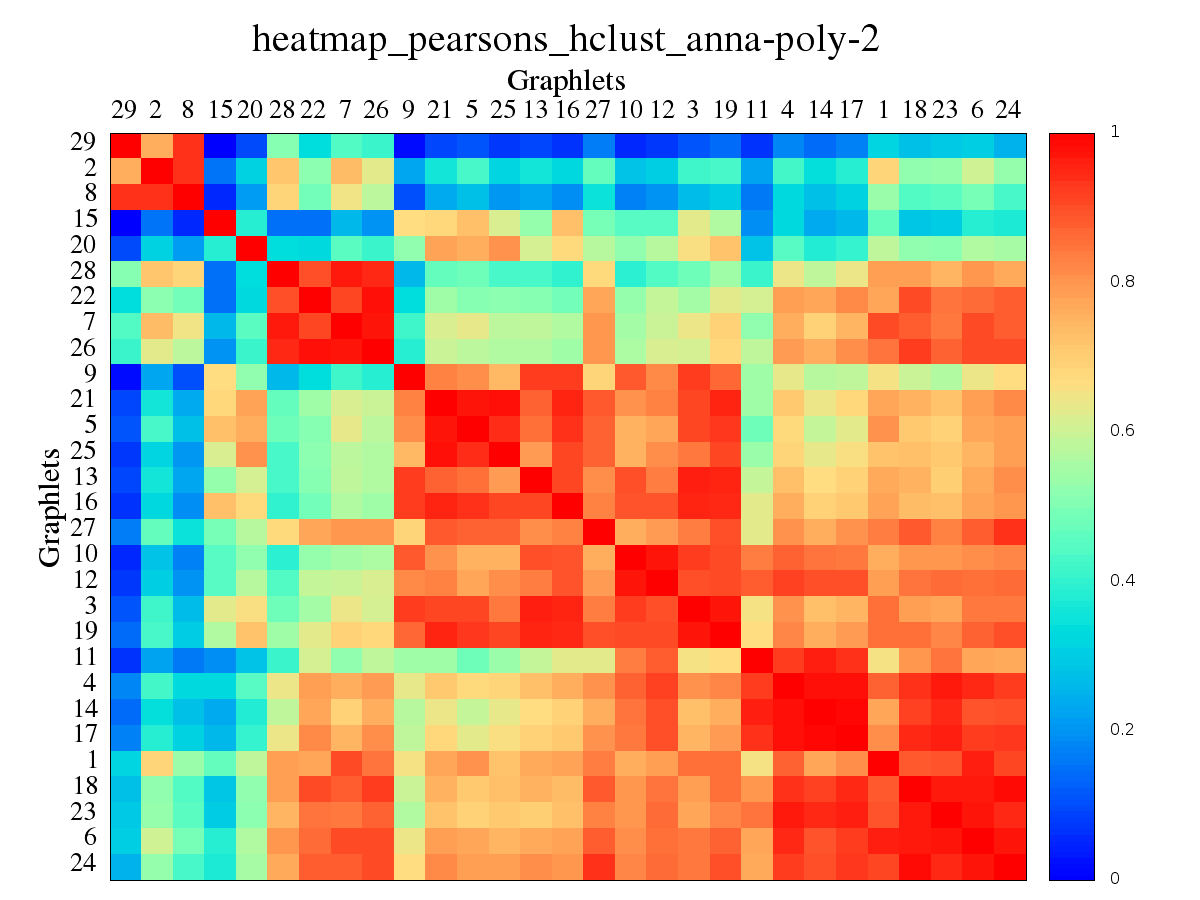
\includegraphics[scale=0.4]
{../code/final_results/knuth_literature/anna/heatmap_pearsons_hclust_anna-poly-2.png}
\caption{}
\label{fig:anna-knuth}
\end{figure}

Cliques 2,8 and 29 cluster with each other. Graphlets 28,22,7 and 26 contain as a subgraph graphlet G7. Graphlets 11,4,14 and 17 all contain claws C4 (graphlet G4).

\subsection*{David Copperfield - Knuth literature}

\begin{figure}[H]
  \centering
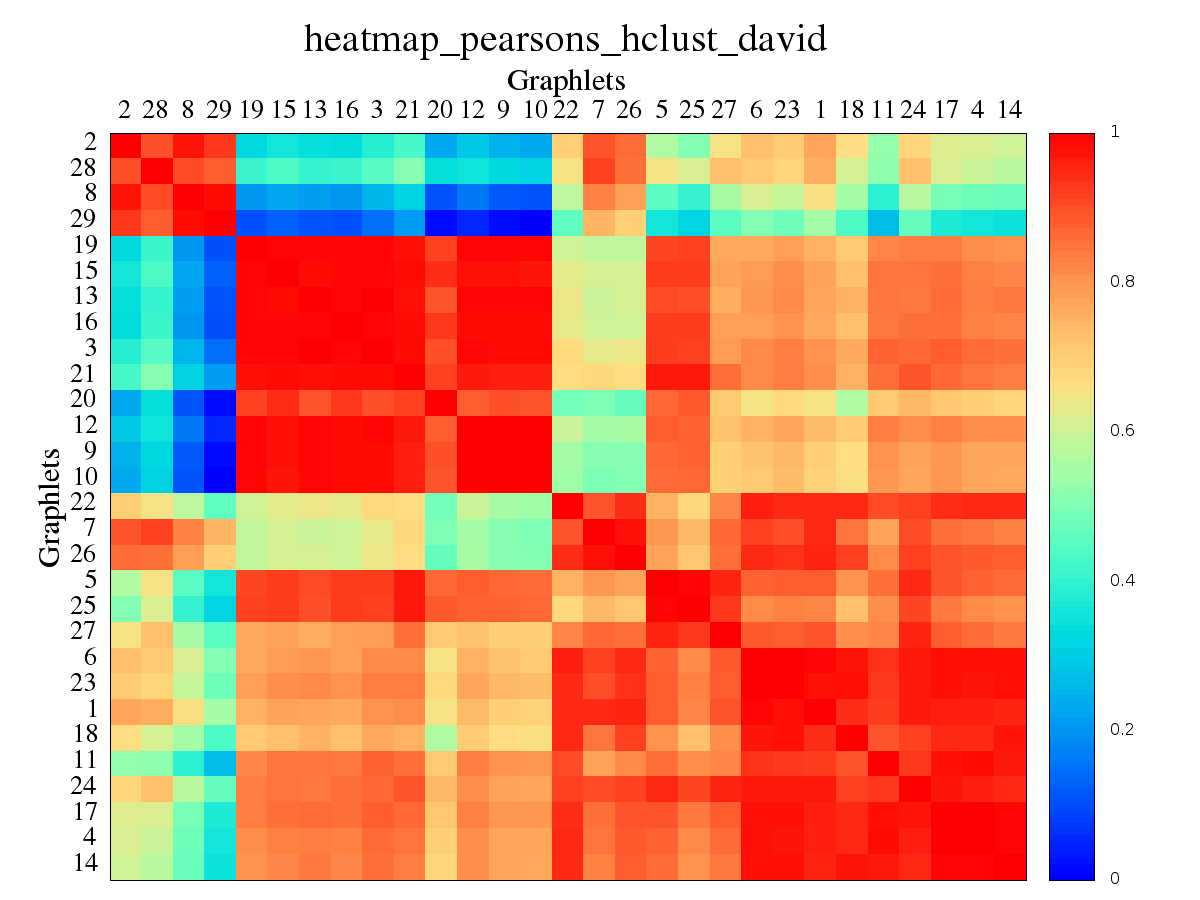
\includegraphics[scale=0.4]
{../code/final_results/knuth_literature/david/heatmap_pearsons_hclust_david.png}
\caption{}
\label{fig:anna-knuth}
\end{figure}

Results for the David Copperfield network are also similar to Anna Karenina: Cliques 2,28,8,29 cluster together. A bigger cluster is formed of Graphlets 19,15,13,16,3,21,20,12,9 and 10 which all contain paths on 4 nodes: P4's (graphlet G3). 


Other literature networks for which I have calculated the heatmaps are:
\begin{itemize}
 \item Knuth Literature:
 \begin{itemize}
    \item Homer - Iliad or Odyssey
    \item Adventures of Huckleberry Finn
    \item Jean (??)
  \end{itemize}
 \item Mreze Literature:
 \begin{itemize}
    \item Anna Karenina
    \item David Copperfield
    \item Les Miserables
  \end{itemize}
  \item Processing under way
  \begin{itemize}
  \item Bible
    \item Old Testament
    \item New Testament
  \end{itemize}
  \end{itemize}

\section*{Conclusion}  
  To conclude, we can clearly say that the main reason for the graphlets clustering together is because they contain as subgraphs the same smaller graphlets. Moreover, the CCA analysis that has been performed on several metabolic, ppi and trade networks has not been able to clearly separate the graphlets into sets with positive and negative weights. The best CCA correlations have been obtained with the trade network (~0.9), followed by some Yeast PPI networks (~0.5) and compounds-based metabolic networks (~0.5). This means that a high correlation (around 90\%) between economic indicators and graphlet GCV signatures can be achieved in the trade network. The reason for the high correlation in the trade network might come as a result of the small size and diameter in this network (119 nodes). 
  
  For the yeast ppi networks, a correlation of around 0.5 indicates that there is some connection between the GCV signature and the 
  ppi annotations. The reason for this might be because the GCV signature only captures some information about the neighbourhood of the protein. Moreover, other differences between proteins might not be due to the way they interact with the environment, but due to their chemical and physical properties.
  

\end{document}
